\documentclass{article}

\usepackage[german]{babel}
\usepackage{array}
\usepackage[letterpaper,top=2cm,bottom=2cm,left=3cm,right=3cm,marginparwidth=1.75cm]{geometry}

\usepackage{amsmath}
\usepackage{graphicx}
\usepackage{subcaption} % Added package
\usepackage[colorlinks=true, allcolors=blue]{hyperref}
\usepackage[T1]{fontenc}
\usepackage{tabularx}
\usepackage{booktabs}


\title{Übungsprotokoll - NWT2 - Übung 03 \\ VLANS}
\author{\vspace{0.5cm} Thomas Brandstätter (s2210239002) \& Jakob Mayr (s2210239021)}

\begin{document}
\maketitle

\section{Konfiguration der Endsysteme}

In der folgenden Übung haben wir die PCs 4.1 und 4.2 benutzt, somit sind die Netze 4.x verwendet worden. Die IP-Konfiguration wird folgendermaßen vergeben: Klick auf „Network“ in der Taskleiste $\rightarrow$ „Network \& Internet Settings“ $\rightarrow$ „Change adapter options“ $\rightarrow$ gewünschtes Netzwerk Interface auswählen, in diesem Fall Ethernet 2 $\rightarrow$ „Properties“ $\rightarrow$ Doppelklick auf „Internet Protocol Version 4“ bzw. „Internet Protocol Version 6“. In den geöffneten Fenstern können wir nun jeweils die IP-Adresse, Subnetzmaske/Präfix und das Gateway eingeben. Folglich sind die Konfigurationen beider PCs zu sehen:

\begin{figure}[!htp]
  \centering
  \begin{minipage}[b]{0.2\textwidth}
    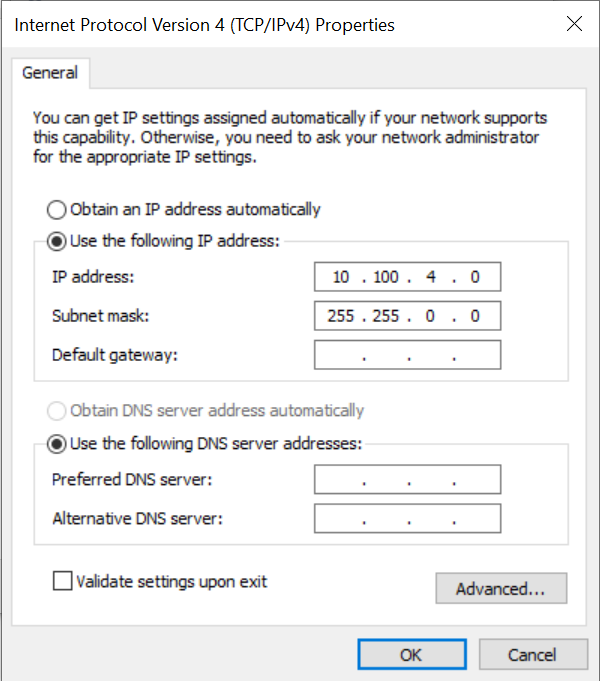
\includegraphics[width=\textwidth]{Arbeitsergebnisse/PC41/pc41_IPv4_config.png}
    \caption{PC41 IPv4 config}
  \end{minipage}
  \hspace{0.8cm}
  \begin{minipage}[b]{0.2\textwidth}
    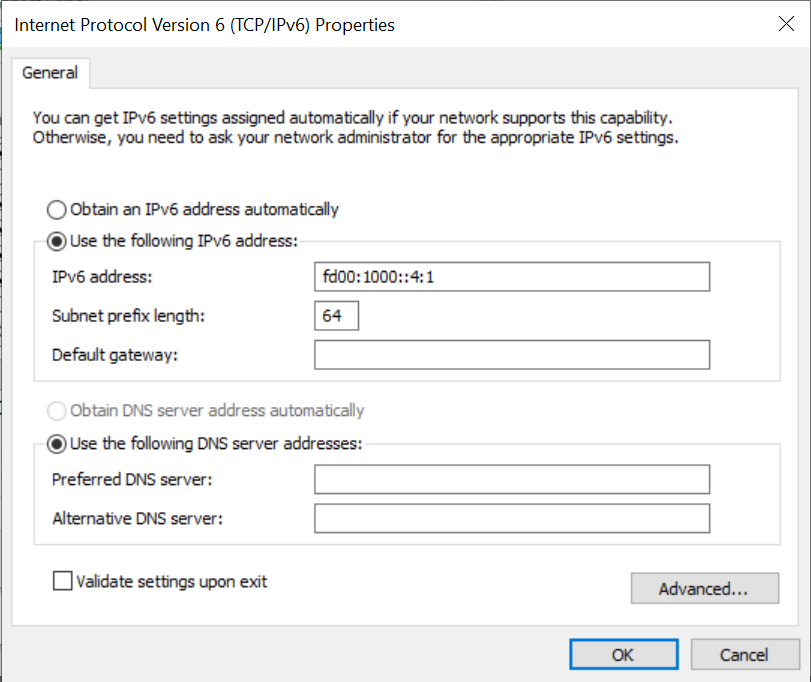
\includegraphics[width=\textwidth]{Arbeitsergebnisse/PC41/pc41_IPv6_config.png}
    \caption{PC41 IPv6 config}
  \end{minipage}
  \hspace{0.8cm}
  \begin{minipage}[b]{0.2\textwidth}
    \includegraphics[width=\textwidth]{Arbeitsergebnisse/PC42/pc42_IPv4_config.png}
    \caption{PC42 IPv4 config}
  \end{minipage}
  \hspace{0.8cm}
  \begin{minipage}[b]{0.2\textwidth}
    \includegraphics[width=\textwidth]{Arbeitsergebnisse/PC42/pc42_IPv6_config.png}
    \caption{PC42 IPv6 config}
  \end{minipage}
\end{figure}

\section{Konfiguration der Gruppenswitches}

Für die Konfiguration des Gruppenswitches wurden für die Clients die Ports FastEthernet0/11 und FastEthernet0/12, für den Backbone-Switch der Port GigabitEthernet0/1 und für den Router der Port GigabitEthernet0/2 verwendet.
Die Ports für die Clients wurden mit dem "access mode" für die VLANS 41 bzw. 42 konfiguriert.

\begin{table}[htbp]
    \centering
    \begin{tabularx}{\textwidth}{>{\bfseries}lX}
        \toprule
        \textbf{Befehl} & \textbf{Erklärung} \\
        \midrule
        switchport access vlan <vlan-tag-numbers> & Mit diesem Befehl wird ein Switchport im „access mode“ einem oder mehreren VLANS zugeordnet. \\
        \hline
        switchport mode access & Mit diesem Befehl wird ein switchport in den „access mode“ gesetzt. \\
        \bottomrule
    \end{tabularx}
    \caption{Verwendete Befehle der Switchports für die Clients}
    \label{tab:commands}
\end{table}

Die Ports für den Backbone-Switch und den Gruppenrouter wurden mit dem „trunk mode“ konfiguriert und haben daher keine zugehörige VLAN-Konfiguration.

\begin{table}[htbp]
    \centering
    \begin{tabularx}{\textwidth}{>{\bfseries}lX}
        \toprule
        \textbf{Befehl} & \textbf{Erklärung} \\
        \midrule
        switchport mode trunk & Mit diesem Befehl wird ein switchport in den „trunk mode“ gesetzt. \\
        \bottomrule
    \end{tabularx}
    \caption{Verwendete Befehle der Switchports für Backbone und Router}
\end{table}

\subsection{Konfiguration der Gruppenrouter}

...

\subsection{Fragen zur Konfiguration}

...

\subsection{Tests und Interpretation ihrer Resultate}

...

\subsection{Konfiguration}

% \bibliographystyle{alpha}
% \bibliography{sample}

\end{document}

